%反函数求导

\pentry{导数\upref{Der}}

\subsection{结论}
若已知 $f(x)$ 的导函数为 $f'(x)$, 则 $f(x)$ 的反函数 ${f^{ - 1}}(x)$ 的导函数为
\begin{equation}
[{f^{ - 1}}(x)]' = \frac{1}{f'[f^{ - 1}(x)]} 
\end{equation} 
为了消除上式可能产生的歧义,记 $f(x)$ 的导函数为 $h(x)$,  $f(x)$ 的反函数为 $g(x)$. 上式变为
 \begin{equation}
g'(x) = \frac{1}{h[g(x)]}
\end{equation}
\subsection{反函数存在的条件}
函数 $y = f(x)$, 在某个区间 $(x_1, x_2)$ 内连续且单调,且 $x$ 与 $y$ 一一对应.因为如果一个 $y$ 有多个 $x$ 对应,反函数中将会出现一个 $x$ 对应多个 $y$ 的情况.
\subsection{反函数的定义}
令满足上述条件的某函数和反函数分别为 $f(x)$,  $g(x)$, 在有定义的区间内的任何一对满足 $y = f(x)$ 的 $x$,  $y$ 都满足 $g(y) = x$, 则 $g(x)$ 是 $f(x)$ 的反函数.

\subsection{证明}
\begin{figure}[ht]
\centering
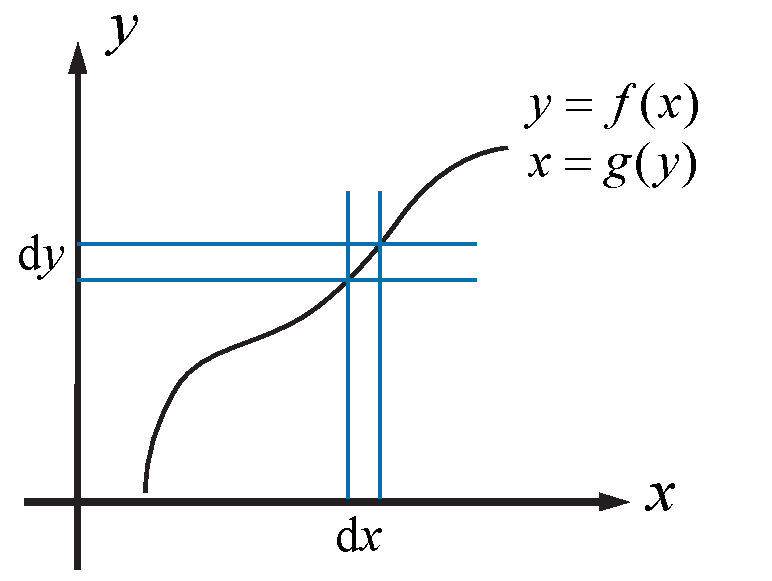
\includegraphics[width=6cm]{./figures/InvDer.pdf}
\caption{在同一点处,$f'=\dv*{y}{x}$, $g'=\dv*{x}{y}$, 互为倒数}\label{InvDer_fig1}
\end{figure}
根据导数和微分的关系, $y = f(x)$ 在 曲线上的某点 $(x_0, y_0)$, 有
 \begin{equation}\label{InvDer_eq1}
\dd{y} = f'(x_0) \dd{x}
\end{equation}
同一点也满足 $g(y_0) = x_0$, 且
 \begin{equation}\label{InvDer_eq2}
g'(y_0)\dd{y} = \dd{x}
\end{equation}
对比\autoref{InvDer_eq1} 和\autoref{InvDer_eq2}, 得
\begin{equation}
g'(y_0) = \dv{x}{y} = \frac{1}{f'(x_0)}
\end{equation}
可见\autoref{InvDer_fig1} 曲线上同一点处 $f'$ 和 $g'$ 互为倒数. 把 ${x_0} = g(y_0)$ 代入上式,得
\begin{equation}
g'(y_0) = \dv{x}{y} = \frac{1}{f'[g(y_0)]}
\end{equation} 
上式中, ${y_0}$ 可以是 $g$ 函数定义域的任意一点,所以
\begin{equation}
g'(y) = \frac{1}{f'[g(y)]}
\end{equation} 
或者用习惯上的 $x$ 作为自变量,得
\begin{equation}
g'(x) = \frac{1}{f'[g(x)]}
\end{equation}
证毕.
















